%!TEX root=masterproef.tex
\subsection{Co\"operatieve algoritmen}
\label{subsection:cooperation}

Het detecteren van abnormaal gedrag, dat op zijn beurt een indicatie kan zijn
van een (poging tot) inbraak door \'e\'en knoop is \'e\'en ding, als netwerk
van knopen tot een consensus komen en met meer zekerheid een verdachte knoop
uitsluiten is een heel ander ding.

Een veel voorkomend onderwerp is dat van co\"operatie tussen knopen, waarbij in
overleg bepaald wordt of en welke andere knoop uitgesloten moet worden uit het
netwerk. In \citep{krontiris2009cooperative} wordt hiertoe eerst langs een
theoretische weg gezocht naar de nodige en voldoende voorwaarden voor
inbraakdetectie. Vervolgens wordt er een praktisch omkaderend algoritme
voorgesteld om op co\"operatieve manier aan inbraakdetectie te doen.

Zowel dit theoretische model als het praktische algoritme vormen een
interessante bron van informatie. Het theoretische model kan helpen bij het
analyseren van andere co\"operatieve oplossingen en het praktische algoritme
biedt een algemeen raamwerk voor het implementeren van co\"operatieve
strategie\"en.

Bijlage \ref{appendix:idp-cooperation} gaat in meer detail in op de
mathematische onderbouw van het zgn. \emph{Intrusion Detection Problem} (IDP).
Naast een theoretisch model wordt tevens een algoritme voorgesteld dat het
mogelijk maakt om op gedistribueerde manier samen te werken en tot een
beslissing te komen aangaande de aanwezigheid van een malafide knoop in het
netwerk.

Het algoritme is een betrekkelijk eenvoudig raamwerk voor een co\"operatieve
aanpak, waarbij knopen zelfstandig beslissen welke andere knopen ze verdenken
en vervolgens gezamenlijk, op een gedistribueerde manier, trachten tot een
consensus te komen welke van de verdachte knopen effectief de aanvaller is.

De kracht van dit raamwerk en het succes ervan hangt natuurlijk sterk af van de
lokale detectiemogelijkheden van de knopen en de accuraatheid hiervan.

\subsubsection*{Risico's}

Het voorbeeld in figuur \ref{fig:idp-examples-2} beslaat een zeer beperkte
scope. We moeten voorzichtig zijn niet te snel conclusies te trekken die in een
ruimere situatie misschien een verkeerd beeld zouden kunnen opleveren. Figuur
\ref{fig:sinkhole-ripple} toont essentieel hetzelfde voorbeeld als dat van
\ref{fig:idp-examples-2}, maar nu met meer knopen rondom het initi\"ele
voorbeeld.

Het routeringalgoritme is gebaseerd op de totale kost van het pad naar het
basisstation en komt daarmee overeen met het MultiHopLQI routering algoritme
beschreven in o.a. \citep{krontiris2008launching}. In dit werk wordt ook de
zgn. \emph{Sinkhole Attack} voorgesteld. We nemen deze aanval als voorbeeld.

\begin{figure}[ht]
\centering
\begin{subfigure}{.49\textwidth}
  \centering
  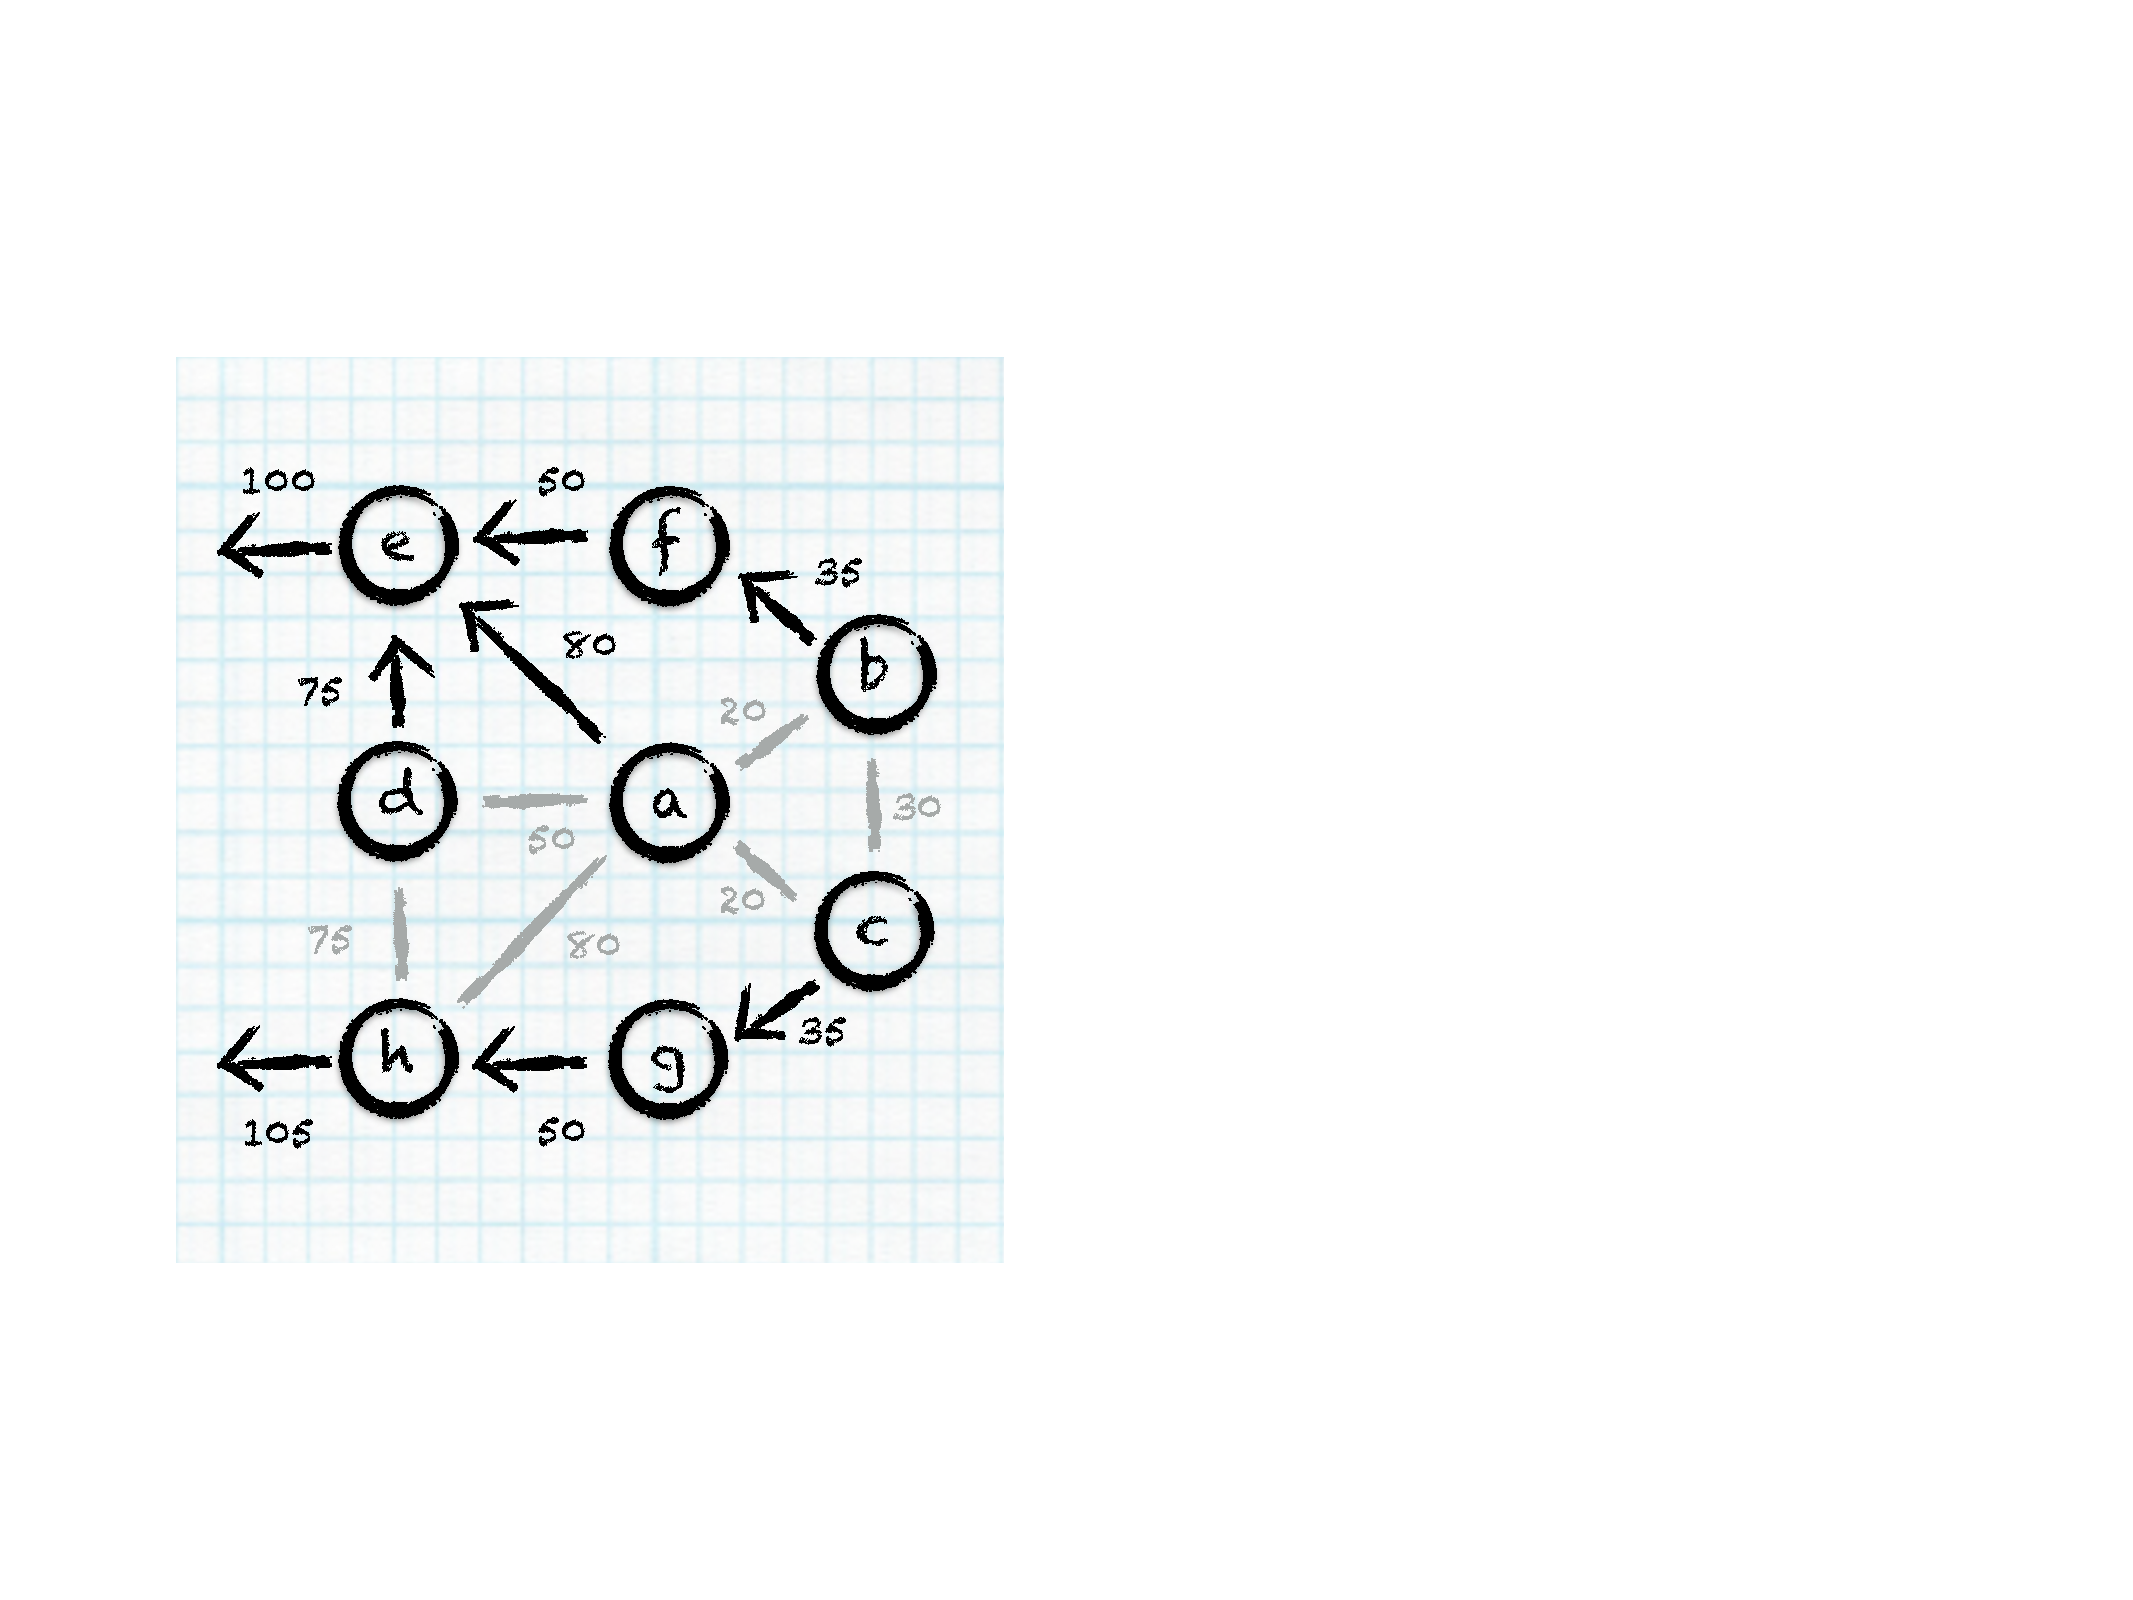
\includegraphics[width=.8\linewidth]{./resources/sinkhole-before.pdf}
  \caption{Initi\"ele topologie, routes en kosten}
  \label{fig:sinkhole-ripple-1}
\end{subfigure}
\begin{subfigure}{.49\textwidth}
  \centering
  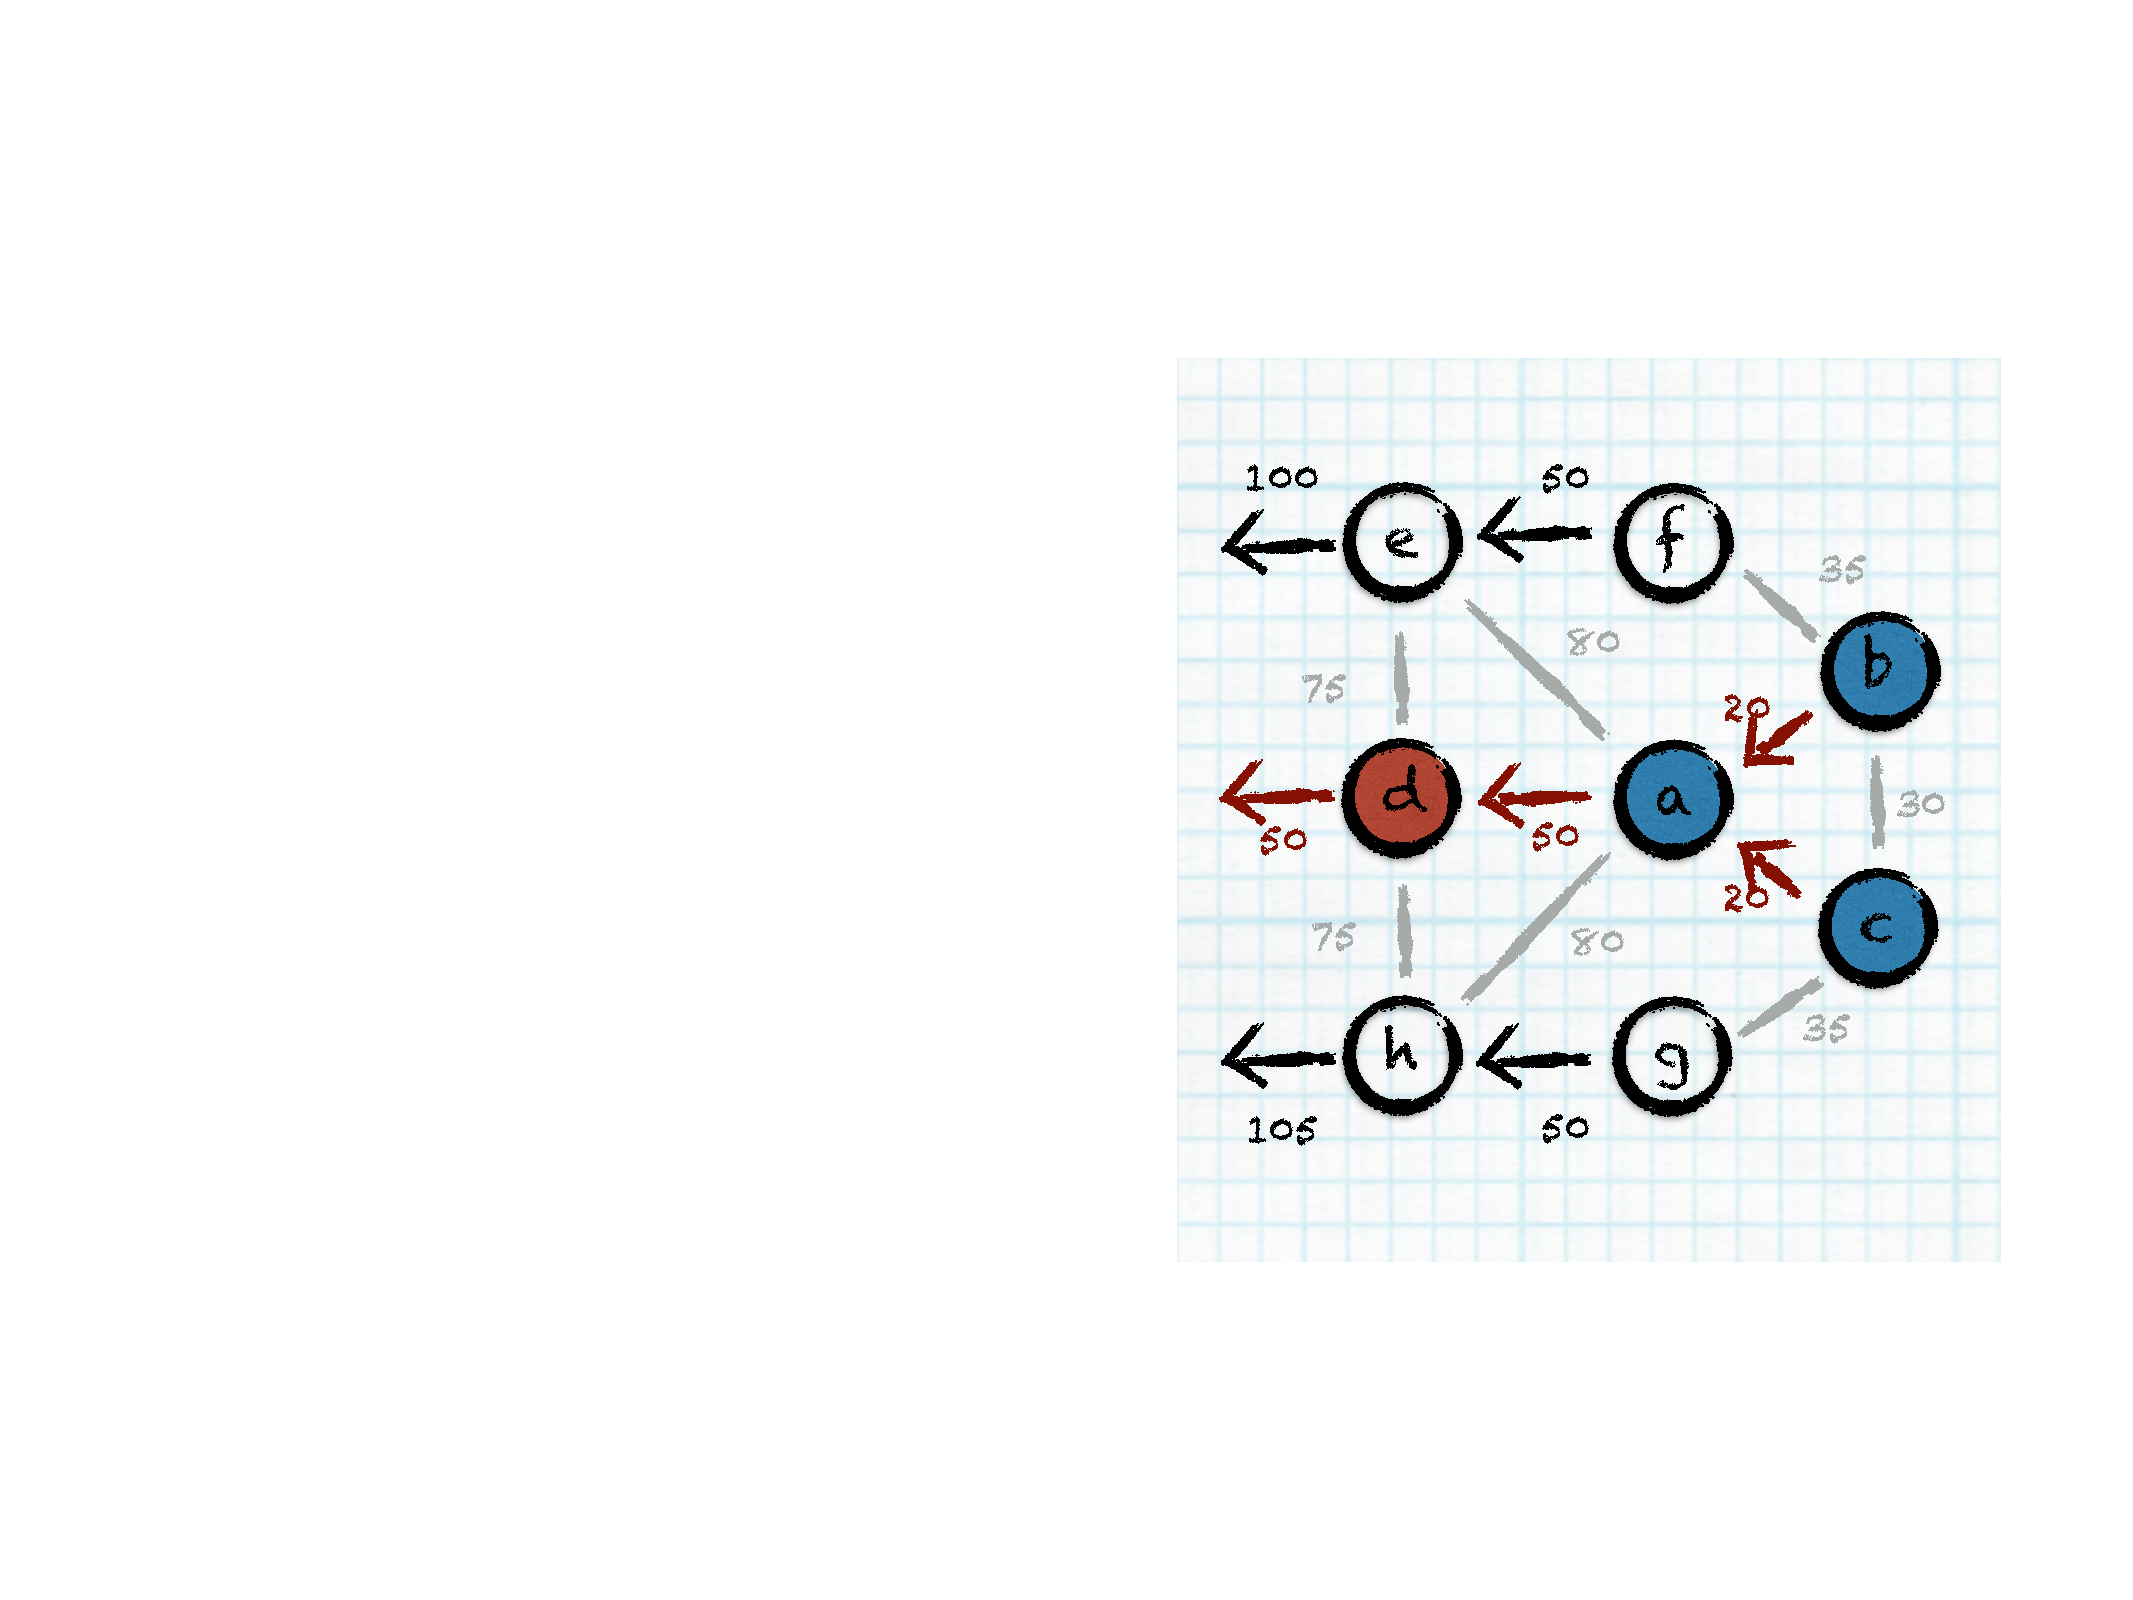
\includegraphics[width=.8\linewidth]{./resources/sinkhole-after.pdf}
  \caption{Knoop $d$ kondigt ``betere'' route aan}
  \label{fig:sinkhole-ripple-2}
\end{subfigure}
\caption{Voorbeeld van het theoretische risico dat kan leiden tot een verkeerde
identificatie van de echte aanvaller}
\label{fig:sinkhole-ripple}
\end{figure}

Stel dat knoop $d$ een \emph{Sinkhole Attack} uitvoert door een zeer lage kost
te adverteren. Hierdoor zal knoop $a$ geneigd zijn om zijn route aan te passen.
Hierdoor zal deze op zijn beurt een veel voordeligere route adverteren en
zullen ook knopen $b$ en $c$ hun route wijzigen en hun gegevens via knoop $a$
versturen.

Ten gevolge van deze route-updates is het mogelijk dat een lokale detector voor
de \emph{Sinkhole Attack} op knopen $a$ en $b$ in werking zal treden. Hierbij
kunnen de knopen alleen hun volledige buurt beschuldigen, omdat het niet
mogelijk is om te detecteren wie de valse boodschappen effectief verstuurd
heeft. Indien de aanvallende knoop $d$ nu ook selectief zijn naburige knoop $a$
beschuldigt, komen we tot dezelfde situatie als in figuur
\ref{fig:idp-examples-2}, echter nu met mogelijk een verkeerd
ge\"identificeerde aanvaller.

Dit voorbeeld is, net zoals de vele andere beschreven voorbeelden, uitermate
specifiek en dient louter ter illustratie van het fragiele karakter van een
co\"operatief algoritme. Desalniettemin bieden de concepten en het omkaderende
algoritme ge\"introduceerd in \citep{krontiris2009cooperative} een goed
uitgangspunt voor het beschrijven en implementeren van
inbraakdetectiemechanismen.

\subsubsection*{Groeperen}
\label{subsubsection:grouping}

Een andere aanpak van co\"operatieve algoritmen vertrekt van het groeperen van
knopen. Deze aanpak wordt toegepast door \citep{li2008group}. Groepering
gebeurt op basis van nabijheid en tracht sensoren te groeperen die door hun
locatie gelijkaardige meetwaarden zouden moeten opmeten. De auteurs stellen een
algoritme voor op basis van verschillen, een zgn. delta-algoritme.

Metingen van knopen kunnen nu binnen de groep met elkaar vergeleken worden, en
afwijkende resultaten (zie ook sectie \ref{subsection:anomaly}) kunnen op
statistische wijze beschouwd worden als abnormaal gedrag en op die manier
gerapporteerd worden.
